% !TEX program = pdflatex
\documentclass[conference,a4paper]{IEEEtran}
\usepackage[utf8]{inputenc}
\usepackage[T5]{fontenc}
\usepackage[vietnamese]{babel}
\IEEEoverridecommandlockouts
\usepackage{amsmath,amssymb,graphicx,booktabs,tabularx,multirow}
\usepackage{float,adjustbox,tikz,pgfplots}
\usetikzlibrary{arrows.meta,positioning,calc}
\pgfplotsset{compat=1.18}
\definecolor{inkblue}{HTML}{193C65}
\definecolor{mutedblue}{HTML}{EAF1F7}
\definecolor{cgreen}{HTML}{296B53}
\definecolor{cred}{HTML}{9D4D45}
\usepackage{xurl}
\usepackage[unicode,hidelinks]{hyperref}
\hypersetup{pdfkeywords={đồ thị cảnh, dự đoán quan hệ, chỉnh sửa đồ thị, nhất quán ngữ nghĩa, quan hệ theo thời gian}}
\usepackage[backend=biber,style=ieee,sorting=none,maxbibnames=4]{biblatex}
\DeclareLanguageMapping{vietnamese}{english}
\DefineBibliographyStrings{vietnamese}{url={Trực tuyến, tại}}
\addbibresource{ref.bib}
\graphicspath{{./}{../latex_report_source/}{../reports/pvsg-trd-m5-v1/}}
\newcommand{\nd}{\textemdash}
\newcommand{\srcnote}[1]{\par\smallskip{\raggedright\footnotesize #1\par}\smallskip}
\newcommand{\reporttodo}[2]{\par\smallskip\noindent\textit{Bằng chứng còn thiếu (#1).} #2\par}
\addto\captionsvietnamese{%
  \renewcommand{\refname}{Tài liệu tham khảo}%
  \renewcommand{\appendixname}{Phụ lục}%
}
\begin{document}
\title{Báo cáo đồ án Học máy với dữ liệu đồ thị\\
Biểu diễn đồ thị ngữ nghĩa cho chỉnh sửa ảnh\\
và dự đoán quan hệ trong video}

\author{%
  \IEEEauthorblockN{%
    \begin{tabular}{@{}c@{\hspace{1.8em}}c@{\hspace{1.8em}}c@{}}
      Nguyễn Đăng Thới Toàn & Hồ Thanh Bình & Dương Thuỷ Tiên\\
      25C15062 & 24C15002 & 24C15026
    \end{tabular}\\[0.6ex]
    \begin{tabular}{@{}c@{\hspace{1.8em}}c@{}}
      Bùi Mạnh Hùng & Nguyễn Đăng Khoa\\
      25C15039 & 25C15046
    \end{tabular}}
  \IEEEauthorblockA{\textit{Khoa Công nghệ thông tin}\\
    \textit{Trường Đại học Khoa học Tự nhiên, ĐHQG TP.HCM}\\
    TP. Hồ Chí Minh, Việt Nam\\
    Giảng viên hướng dẫn: TS. Lê Ngọc Thành và ThS. Huỳnh Lâm Hải Đăng}}

\maketitle
\pagestyle{plain}
\thispagestyle{plain}
\begin{abstract}
Đồ án dùng đồ thị cảnh để trả lời ba câu hỏi: quan hệ nào tồn tại giữa hai đối tượng,
cần sửa thành phần nào của đồ thị theo câu lệnh và ảnh sau chỉnh sửa có giữ đúng
nội dung yêu cầu hay không. Trên VG150, GAT tăng 1,65 điểm phần trăm mR@50 so
với MLP. Điều chỉnh hàm mất mát theo tần suất lớp tăng 6,48 điểm khi tắt tri thức
nền. Ở bài toán biến đổi đồ thị, GNN đạt micro-F1 7,34\% trên MagicBrush và
82,44\% trên bộ cặp đồ thị có cấu trúc EMNLP 2020. Trên 200 yêu cầu chỉnh sửa ảnh,
điểm nhất quán đồ thị đánh giá được 45,5\% số cặp, với tương quan Spearman 0,1767
so với nhãn người trên tập có điểm. Phần mở rộng video kiểm tra dự đoán quan hệ
và thời gian trên track chuẩn của PVSG. Trong tám cấu hình, Temporal Conv đạt
R@50 cao nhất (8,63\%), còn ST-GAT đạt mR@50 cao nhất (2,38\%).
\end{abstract}

\section{Giới thiệu}
Một yêu cầu như “thêm con mèo dưới gốc cây” xác định cả đối tượng cần thêm, vị trí tương đối và phần cảnh cần giữ. Đồ thị cảnh biểu diễn hai đối tượng bằng đỉnh và quan hệ có hướng bằng cạnh. Đồ án chọn nhánh ảnh tĩnh làm bài toán chính. Các mô hình thị giác và sinh ảnh được dùng ở chế độ
đóng băng; phần học là các mô hình trên đồ thị. Bảng~\ref{tab:scorecard} tổng hợp
kết quả trước khi đi vào thiết lập, đối chứng và phân tích lỗi.

\begin{table*}[!t]\centering\small
\caption{Kết quả chính của ba nhiệm vụ và thực nghiệm mở rộng. Các hàng khác dataset, split hoặc metric không dùng để xếp hạng chung.}\label{tab:scorecard}
\begin{tabularx}{\linewidth}{@{}p{10mm}p{28mm}p{29mm}X@{}}
\toprule NV & Phần & Dữ liệu / split & Kết quả chính\\\midrule
1 & Relation prediction & VG150 / test & GAT mR@50 \textbf{18,61\%}; hơn MLP \textbf{1,65 pp}.\\
1 & Loss ablation & VG150 / test & Adjusted, KG-off: mR@50 \textbf{24,59\%}, tăng \textbf{6,48 pp} so CE-off.\\
1 & KG fusion & VG150 / test & Pair-real mR@50 \textbf{25,24\%}; hơn shuffled 0,24 pp, chỉ 2/3 seed tăng.\\
2A & Phương pháp 2023+ & Custom GQA / test & PE-PLPR mR@50 \textbf{4,07\%}.\\
2A & AlignG ablation & Custom GQA / test & GC mR@50: \textbf{4,07 $\to$ 4,62\%}; bản adapted.\\
2B & Biến đổi đồ thị gốc & MagicBrush / test & GNN micro-F1 \textbf{7,34\%}; exact target graph \textbf{0\%}.\\
2B & Dataset thay thế & EMNLP 2020 / test & GNN micro-F1 \textbf{82,44\%}; macro-F1 \textbf{55,03\%}.\\
3 & Nhất quán đồ thị & VN100 / 200 edit & $\rho_G=\mathbf{0,1767}$; coverage \textbf{45,5\%}.\\
3 & Baseline ảnh & Tập giao $N=91$ & $-\mathrm{LPIPS}$ 0,1962; Graph 0,1767; CLIPScore 0,0561.\\
Video & Quan hệ video & PVSG / test & Conv kernel 5 đạt R@50 \textbf{8,63\%}; ST-GAT đạt mR@50 \textbf{2,38\%} trên track chuẩn.\\
\bottomrule\end{tabularx}
\end{table*}

\subsection{Quy ước đọc kết quả}
R và mR là phần trăm; pp là \emph{điểm phần trăm}, không phải phần trăm tăng
tương đối. Mean $\pm$ std là trung bình và độ lệch chuẩn mẫu qua ba seed,
không phải khoảng tin cậy. GC (graph constraint) giữ một predicate cho mỗi cặp
object có hướng; NG cho phép nhiều predicate. Bảng VG150 chính dùng GC
reference-v1 trên 26.446 ảnh test. Long-tail và zero-shot cũng đã bổ sung
kết quả test; custom GQA có cả tập validation và tập test của đồ án. Các ca định tính VG150 dùng validation.

\subsection{Ba kết luận cần kiểm chứng}
\begin{enumerate}
\item \textbf{Nhiệm vụ 1:} GAT có lợi so với MLP, nhưng điều chỉnh loss
tác động tới mR lớn hơn các cách thêm KG đã thử. Tăng mR không đồng nghĩa tăng R.
\item \textbf{Nhiệm vụ 2:} phương pháp mới tăng mR trên custom GQA; học graph operation
khả thi hơn khi supervision có cấu trúc. EMNLP không thay thế bằng chứng còn thiếu
của pipeline từ ảnh MagicBrush.
\item \textbf{Nhiệm vụ 3:} điểm đồ thị cung cấp chẩn đoán theo object/quan hệ nhưng
độ phủ thấp. Tương quan hiện tại chưa chứng minh ưu thế so với baseline ảnh.
\end{enumerate}
\srcnote{Nguồn số liệu: các report versioned trong \path{reports/level1}, \path{reports/level2}
và \path{docs/LEVEL3_RESULTS_V1.md}. Ánh xạ chi tiết nằm trong \path{SOURCE_MAP.md} đi kèm.}

\section{Nhiệm vụ 1. Dự đoán quan hệ trong đồ thị cảnh}

\subsection{Bài toán và đầu vào, đầu ra}
Trong Hình~\ref{fig:motifs}, một phụ nữ và một chiếc xe máy đã được khoanh vùng.
Biết hai đối tượng này có mặt trong ảnh vẫn chưa đủ để mô tả cảnh. Quan hệ
\textit{riding} (đang cưỡi) cho biết người phụ nữ đang làm gì với chiếc xe.
Trong đồ thị cảnh, hai đối tượng là hai đỉnh, còn quan hệ này là một cạnh có
hướng từ người phụ nữ đến xe máy.

\begin{figure}[!ht]
\centering
\includegraphics[width=.83\columnwidth]{neural-motifs-fig1.pdf}
\caption{Minh họa đầu vào và đích dự đoán. Phía trên là ảnh và các hộp đối tượng.
Phía dưới là đồ thị chú thích, trong đó có bộ ba
\textit{woman--riding--motorcycle}. Trích Hình~1, trang~1 của
Zellers và cộng sự~\cite{zellers2018neuralmotifs}.}
\label{fig:motifs}
\end{figure}

Nhóm xét bài toán phân lớp quan hệ (\textit{Predicate Classification}, PredCls).
\textbf{Đầu vào} gồm ảnh RGB, hộp bao và nhãn lớp thật của từng đối tượng.
\textbf{Đầu ra} là danh sách bộ ba (đối tượng chủ thể, quan hệ, đối tượng đích),
kèm điểm tin cậy. Hai đối tượng được xác định theo từng hộp cụ thể. Một ảnh có
$N$ đối tượng tạo ra $N(N-1)$ cặp có hướng cần xét. Mô hình tự xác định cặp
nào có quan hệ và dự đoán nhãn cho cặp đó. Các cạnh có nhãn trong đồ thị
chú thích chỉ được dùng để huấn luyện và chấm kết quả.

\subsection{Dữ liệu và cách đánh giá}
VG150 là tập con của Visual Genome~\cite{krishna2017visualgenome}, gồm
150 lớp đối tượng và 50 lớp quan hệ. Nhóm chia dữ liệu theo ảnh. Sau khi
đối chiếu metadata và giữ những ảnh có hộp cùng chú thích quan hệ, nhóm
lấy 5.000 ảnh hợp lệ đầu tiên theo thứ tự lưu trong phần train làm
validation, giữ 57.723 ảnh còn lại để huấn luyện và giữ 26.446 ảnh hợp lệ
từ phần test để đánh giá. Các cặp đối tượng của một ảnh luôn thuộc cùng một tập.

Mỗi cặp có 51 điểm đầu ra, gồm 50 quan hệ và lớp nền. Khi đánh giá với
\textit{graph constraint} (GC), nhóm giữ quan hệ có xác suất cao nhất trong
50 quan hệ của mỗi cặp, sau đó xếp hạng tất cả các cặp trong cùng ảnh.
Một dự đoán khớp chú thích khi đúng nhãn quan hệ, đúng hai lớp đối tượng theo
thứ tự và độ giao trên hợp (IoU) của từng hộp với hộp chuẩn đạt ít nhất 0,5.

\textbf{R@50} đo tỷ lệ quan hệ chuẩn được tìm lại trong 50 dự đoán đứng đầu
của mỗi ảnh, rồi lấy trung bình qua ảnh. \textbf{mR@50} tính recall theo ảnh
cho từng loại quan hệ có mặt, rồi lấy trung bình trên 50 lớp. Vì vậy, một
lượt tìm lại quan hệ hiếm có thể ít ảnh hưởng đến R@50 nhưng có ý nghĩa khi
xét mR@50. Toàn bộ bảng định lượng dùng cùng bộ chấm \textit{reference-v1}
trên test. Nhóm chấm lại các checkpoint đã chọn bằng validation. Tập test
này đã từng được đánh giá bằng bộ chấm trước đó.

\subsection{Hai mô hình cơ sở}
Mỗi đỉnh có vector 549 chiều. Vector gồm 512 chiều thị giác trích từ vùng
ảnh bằng CLIP ViT-B/32 đóng băng~\cite{radford2021clip}, năm số hình học
(tọa độ tâm, chiều rộng, chiều cao, diện tích đã chuẩn hóa) và 32 chiều
biểu diễn nhãn đối tượng học trong khi huấn luyện. Hai mô hình ở
Hình~\ref{fig:vg-arch} dùng cùng đầu vào và chấm cùng tập cặp.

\begin{figure}[!ht]
\centering
\begin{tikzpicture}[>=Latex,font=\footnotesize,align=center,
 box/.style={draw=inkblue,rounded corners=2pt,inner sep=4pt},
 model/.style={box,text width=.39\columnwidth,minimum height=12mm}]
\node[box] (x) {Đặc trưng từng đối tượng (549 chiều)};
\node[model,below left=5mm and 1mm of x.south] (m) {MLP\\Ghép chủ thể và đích};
\node[model,below right=5mm and 1mm of x.south] (g) {GAT\\Truyền tin trên đồ thị,\\rồi ghép chủ thể và đích};
\node[box,below=24mm of x.south] (y) {51 điểm cho mỗi cặp có hướng};
\draw[->] (x.south) -- (m.north);
\draw[->] (x.south) -- (g.north);
\draw[->] (m.south) -- (y.north);
\draw[->] (g.south) -- (y.north);
\end{tikzpicture}
\caption{Hai đường dự đoán quan hệ. Thứ tự chủ thể và đối tượng đích được
giữ khi ghép vector. Với GAT, đặc trưng của mỗi đỉnh còn phụ thuộc các đỉnh
khác trong cùng ảnh.}
\label{fig:vg-arch}
\end{figure}

\textbf{MLP.} Ghép hai vector theo thứ tự chủ thể và đích thành vector 1.098
chiều. Hai lớp tuyến tính có kích thước $1.098\to256\to51$, với ReLU ở giữa,
tạo điểm quan hệ chỉ từ cặp đang xét.

\textbf{GAT.} Mô hình chiếu mỗi đỉnh từ 549 xuống 256 chiều, sau đó dùng
hai lớp graph attention~\cite{velickovic2018gat}, mỗi lớp bốn đầu chú ý.
Cạnh truyền tin nối mọi cặp đối tượng khác nhau trong ảnh và có vòng tự nối (\textit{self-loop}).
Tại mỗi lớp, đỉnh tổng hợp thông tin từ các đỉnh lân cận theo trọng số chú ý.
Hai vector sau truyền tin được ghép thành 512 chiều và đi qua bộ phân lớp
$512\to256\to51$. Mô hình dùng dropout 0,1.

\textbf{Huấn luyện.} Nhóm dùng AdamW với tốc độ học $10^{-3}$, weight decay
$10^{-2}$, batch hiệu dụng 512 ảnh, tối đa 200 epoch và dừng sớm với
patience 15. Mỗi cặp dương được lấy kèm tối đa ba cặp nền. Vì hàm mất mát
nhận một nhãn đích, bộ lấy mẫu bỏ qua các cặp có nhiều nhãn quan hệ khác nhau
khi train. Bộ chấm vẫn giữ các chú thích này. Nhóm đánh giá 54 checkpoint, tương ứng 18 cấu hình, mỗi cấu hình chạy với ba seed
42, 123 và 3407.

\subsection{Điều chỉnh hàm mất mát và bổ sung tri thức nền}
\textbf{Điều chỉnh theo tần suất lớp.} Mười loại quan hệ phổ biến nhất chiếm
88,40\% chú thích quan hệ trong tập train. Để giảm thiên lệch về những lớp
này, nhóm so sánh cross-entropy (CE) với \textit{logit-adjusted loss} theo công thức
\[
\mathcal{L}_{\mathrm{adj}}(z,y)=\operatorname{CE}(z+0{,}25\log\pi,\,y).
\]
Ở đây $z$ là vector điểm trước softmax, $y$ là nhãn đích và $\pi$ là phân bố
lớp ước lượng từ train theo quy tắc lấy mẫu, có cộng một vào số đếm mỗi lớp.
Vì $\log\pi$ âm hơn với lớp hiếm, mô hình phải học điểm $z$ cao hơn cho lớp
đó để dự đoán đúng khi train. Khi suy luận, nhóm xếp hạng từ điểm $z$ gốc.

\textbf{Tri thức tại đỉnh.} Nhóm liên kết nhãn đối tượng với khái niệm trong
WordNet hoặc ConceptNet~\cite{miller1995wordnet,speer2017conceptnet}. Với nhãn
có liên kết, nhóm ghép một vector tri thức 64 chiều đã đóng băng và một cờ
hợp lệ vào đặc trưng đỉnh. WordNet liên kết được 150/150 lớp, ConceptNet
liên kết được 138/150 lớp. Nhóm dùng TransE cho cả hai nguồn, đồng thời thử
RotatE và ComplEx trên ConceptNet~\cite{bordes2013transe,sun2019rotate,trouillon2016complex}.

\textbf{Tri thức tại cặp.} Với \textit{pair fusion}, hai vector tri thức của
chủ thể và đích tạo ra phần hiệu chỉnh cộng vào điểm quan hệ của GAT.
Một cổng học được điều khiển biên độ hiệu chỉnh. Với \textit{visual fusion},
cổng còn nhận đặc trưng GAT của hai đối tượng trong ảnh và điều tiết riêng
cho từng quan hệ. Để kiểm tra vai trò của ánh xạ lớp--khái niệm, nhóm giữ
cùng kiến trúc và tráo vector giữa 138 lớp ConceptNet có liên kết hợp lệ
(\textit{shuffled-KG}). Cả ba seed huấn luyện dùng cùng một hoán vị cố định.

\subsection{Kết quả chính và phân tích ablation}
\begin{table}[!ht]
\centering\small
\caption{Dự đoán quan hệ trên 26.446 ảnh test VG150. Điểm là phần trăm,
trung bình $\pm$ độ lệch chuẩn mẫu của ba seed. Mỗi nhóm có đối chứng riêng.}
\label{tab:vgscore}
\begin{tabular}{@{}lrr@{}}\toprule
Cấu hình & R@50 & mR@50\\\midrule
\multicolumn{3}{@{}l}{\textit{Mô hình cơ sở và tri thức tại đỉnh}}\\
MLP & $63{,}56\pm0{,}77$ & $16{,}95\pm1{,}52$\\
GAT & $63{,}87\pm0{,}73$ & $18{,}61\pm0{,}25$\\
GAT nhánh WordNet, tắt KG & $63{,}89\pm0{,}38$ & $18{,}44\pm0{,}29$\\
WordNet--TransE & $64{,}15\pm0{,}29$ & $17{,}84\pm0{,}09$\\
WordNet--TransE, bỏ cạnh & $64{,}11\pm1{,}15$ & $18{,}41\pm0{,}90$\\
ConceptNet--TransE & $64{,}10\pm0{,}27$ & $18{,}39\pm0{,}29$\\
ConceptNet--TransE, bỏ cạnh & $64{,}59\pm0{,}19$ & $18{,}15\pm0{,}28$\\
ConceptNet--RotatE & $64{,}21\pm0{,}37$ & $18{,}57\pm0{,}42$\\
ConceptNet--ComplEx & $64{,}37\pm0{,}18$ & $18{,}33\pm0{,}24$\\\midrule
\multicolumn{3}{@{}l}{\textit{Hàm mất mát $\times$ tri thức tại cặp}}\\
CE, tắt KG & $64{,}42\pm0{,}10$ & $18{,}11\pm0{,}16$\\
CE, bật KG & $63{,}63\pm0{,}14$ & $19{,}27\pm0{,}75$\\
Adjusted, tắt KG & $62{,}18\pm0{,}16$ & $24{,}59\pm0{,}93$\\
Adjusted, bật KG & $62{,}01\pm0{,}31$ & $24{,}67\pm1{,}07$\\\midrule
\multicolumn{3}{@{}l}{\textit{Fusion với adjusted loss}}\\
GAT, tắt nhánh hiệu chỉnh & $62{,}06\pm0{,}39$ & $24{,}32\pm0{,}91$\\
Pair, KG thật & $62{,}37\pm0{,}19$ & $\mathbf{25{,}24\pm0{,}39}$\\
Pair, KG xáo trộn & $62{,}34\pm0{,}18$ & $25{,}00\pm0{,}71$\\
Visual, KG thật & $62{,}34\pm0{,}21$ & $24{,}52\pm0{,}64$\\
Visual, KG xáo trộn & $62{,}20\pm0{,}23$ & $24{,}82\pm1{,}25$\\
\bottomrule\end{tabular}
\end{table}

Trên cùng đặc trưng CLIP, GAT tăng mR@50 so với MLP ở cả ba seed, trung bình
1,65 điểm phần trăm. R@50 tăng 0,31 điểm (Bảng~\ref{tab:vgscore}).
Để xác định thành phần nào tạo nên chênh lệch, nhóm lần lượt thay một yếu tố
trong từng họ mô hình. Bảng~\ref{tab:vgdelta} ghi hiệu số ghép cặp theo seed,
tính trước khi làm tròn.

\begin{table}[!ht]
\centering\small\setlength{\tabcolsep}{3pt}
\caption{Ablation trên VG150 test. Dấu dương biểu thị cấu hình bên trái
cao hơn đối chứng bên phải. Các độ chênh tính bằng điểm phần trăm.}
\label{tab:vgdelta}
\begin{tabularx}{\columnwidth}{@{}Xrr@{}}\toprule
Phép so sánh & $\Delta$R@50 & $\Delta$mR@50\\\midrule
WordNet tại đỉnh: bật KG trừ tắt KG & $+0{,}26$ & $-0{,}60$\\
WordNet: giữ cạnh trừ bỏ cạnh & $+0{,}04$ & $-0{,}57$\\
ConceptNet: giữ cạnh trừ bỏ cạnh & $-0{,}49$ & $+0{,}24$\\
Adjusted trừ CE, tắt KG tại cặp & $-2{,}24$ & $+6{,}48$\\
Adjusted trừ CE, bật KG tại cặp & $-1{,}61$ & $+5{,}40$\\
Bật trừ tắt KG tại cặp, adjusted loss & $-0{,}17$ & $+0{,}09$\\
Pair: KG thật trừ tắt hiệu chỉnh & $+0{,}31$ & $+0{,}93$\\
Pair: KG thật trừ KG xáo trộn & $+0{,}02$ & $+0{,}24$\\
Visual: KG thật trừ KG xáo trộn & $+0{,}14$ & $-0{,}30$\\
\bottomrule\end{tabularx}
\end{table}

\textit{(1) Ghép KG tại đỉnh.} Khi giữ cấu hình WordNet--TransE và bật vector
tri thức, mR@50 giảm ở cả ba seed. Như vậy độ phủ liên kết 150/150 lớp vẫn
chưa đủ để cải thiện khả năng nhận biết quan hệ theo lớp.

\textit{(2) Truyền tin giữa các đối tượng.} Thí nghiệm \textit{edges-off} bỏ
cạnh giữa các đỉnh, giữ self-loop và giữ nguyên toàn bộ cặp cần chấm điểm.
Giữ cạnh giúp ConceptNet--TransE tăng 0,24 điểm mR@50, trong khi WordNet--TransE
giảm 0,57 điểm. Tác dụng của ngữ cảnh đồ thị phụ thuộc cách biểu diễn đỉnh.

\textit{(3) Loss và KG.} Trong thiết kế $2\times2$, thay CE bằng adjusted
loss tăng mR@50 cả khi tắt lẫn khi bật KG tại cặp. Khi đã dùng adjusted
loss, bật thêm KG chỉ tăng trung bình 0,09 điểm và có một seed giảm.
Thay đổi lớn nhất trong nhóm đối chứng này đến từ điều chỉnh loss, đi kèm
đánh đổi về R@50.

\textit{(4) Nội dung tri thức trong fusion.} Pair fusion với KG thật đạt
mR@50 cao nhất trong 18 cấu hình. So với đối chứng tráo vector, lợi thế
chỉ còn 0,24 điểm, với hai seed tăng và một seed giảm. Visual fusion cho
chênh lệch theo chiều ngược lại. Với ba seed và một hoán vị, lợi ích riêng
của việc gắn đúng tri thức cho từng lớp còn chưa ổn định.

\subsection{Quan hệ hiếm và phân tích lỗi}
\textbf{Quan hệ nào được cải thiện?} Nhóm xếp 50 quan hệ theo số lần xuất hiện
trong train, rồi chia thành 10 lớp phổ biến, 20 lớp trung bình và 20 lớp hiếm.
Ở hai cấu hình cùng tắt KG, thay CE bằng adjusted loss làm mR@50 của nhóm
trung bình tăng từ 16,19 lên 26,56\%, nhóm hiếm tăng từ 3,54 lên 9,55\%,
còn nhóm phổ biến giảm từ 51,10 xuống 50,72\%. Kết quả này giải thích vì sao
recall trung bình theo lớp tăng rõ dù recall trung bình theo ảnh giảm.

\textbf{Bộ ba chưa gặp trong train.} Tập test chứa 7.848 chú thích trên
4.660 ảnh có tổ hợp (lớp chủ thể, quan hệ, lớp đích) chưa xuất hiện trong
chú thích train. Nhóm giữ cách xếp hạng toàn ảnh và tính recall riêng cho
các chú thích này (zR@50). Với cùng quy tắc GC, chín checkpoint thuộc ba cấu
hình fusion đạt trung bình 11,71\% khi tắt hiệu chỉnh, 11,43\% với KG thật
tại cặp và 11,26\% với KG xáo trộn. Ưu thế mR@50 của pair fusion trên toàn
tập vì thế chưa chuyển thành ưu thế trên các tổ hợp mới.

\begin{figure}[!ht]
\centering
\includegraphics[width=.48\columnwidth]{hit03.png}\hfill
\includegraphics[width=.48\columnwidth]{miss03.png}
\caption{Hai cặp trong cùng ảnh validation số 89, chấm bằng GAT seed 42.
Hộp đỏ đánh dấu chủ thể, hộp xanh đánh dấu đối tượng đích. Trái:
\textit{flower--in--vase}, hạng 1. Phải: \textit{shelf--on--table}, hạng 64.}
\label{fig:vg-paired}
\end{figure}

\textbf{Một ảnh, hai kết quả.} Ở Hình~\ref{fig:vg-paired}, GAT chọn đúng
nhãn cho cả hai cặp, nhưng chỉ bộ ba ở hạng 1 được tính trúng trong top-50.
Bộ ba ở hạng 64 được thu hồi khi tăng ngưỡng lên 100. Một cơ chế bỏ sót khác
xuất hiện ở ảnh số 3. Cặp \textit{girl--hair} có cả hai nhãn chuẩn \textit{has}
và \textit{with}. GC chỉ giữ \textit{with}. Hai ví dụ cho thấy cần xem cả
điểm xếp hạng và số nhãn chuẩn của cặp trước khi quy lỗi cho bộ phân lớp.
Phụ lục~\ref{app:vgcases} liệt kê đủ năm trường hợp trúng và năm trường hợp
bỏ sót đã chọn trên validation.

\section{Nhiệm vụ 2. Phương pháp mới và biến đổi đồ thị}
\subsection{Task A. Dự đoán quan hệ trên GQA}

Task A áp dụng lại bài toán PredCls của Nhiệm vụ 1 trên dataset thứ hai,
GQA~\cite{hudson2019gqa}. Với bounding box và nhãn đối tượng đã biết, mô hình
vẫn dự đoán predicate cho từng cặp có hướng. Trên GQA, nhóm khảo sát liệu
việc biểu diễn mỗi predicate bằng một vector đại diện (\textit{prototype})
có giúp nhận diện quan hệ trên nhiều lớp hơn hay chủ yếu cải thiện recall
trên toàn ảnh.

\subsubsection{Dataset và split}
Nhóm chia phần train chính thức theo ảnh thành 69.942 ảnh train và
5.000 ảnh validation, dùng 10.696 ảnh từ phần validation chính thức làm
test của đồ án. Vocabulary xây từ annotation của riêng tập train có
310 foreground predicates. Hình~\ref{fig:gqa-train-predicates} cho thấy
hai quan hệ trái/phải chiếm 89,16\% số chú thích train, trong khi 42 lớp
có dưới 20 chú thích mỗi lớp. Phân bố tương tự xuất hiện trên test. Hai nhãn
\textit{to the left of} và \textit{to the right of} chiếm tổng cộng
476.716 trong 534.437 chú thích quan hệ (89,2\%). R@$K$ đo tỷ lệ
quan hệ chuẩn được tìm thấy trong top-$K$ của từng ảnh rồi lấy trung bình
trên 10.298 ảnh có quan hệ chuẩn. Vì vậy, trên ảnh có nhiều chú thích
trái/phải, tìm đúng hai quan hệ này có thể đem lại R@$K$ cao dù mô hình
bỏ sót các predicate khác. Với mR@$K$, nhóm tính recall theo ảnh cho từng
predicate rồi lấy trung bình đều trên 310 lớp. Hai lớp trái/phải chỉ chiếm
$2/310$ trọng số của mR@$K$. Có 15 lớp vắng trong test được tính recall bằng 0.

\begin{figure}[!ht]\centering
\begin{tikzpicture}
\begin{semilogyaxis}[report plot,width=.98\linewidth,height=5.4cm,
 xmin=0,xmax=315,ymin=1,ymax=4000000,xtick={1,100,200,310},
 ytick={1,100,10000,1000000},ymajorgrids,
 xlabel={Hạng quan hệ trên tập train},ylabel={Số chú thích (log)}]
\path[fill=mutedblue] (axis cs:268.5,1) rectangle (axis cs:310.5,4000000);
\draw[dashed,cred] (axis cs:1,20)--(axis cs:310,20);
\addplot[inkblue,thin,mark=*,mark size=.42pt] table[x=rank,y=count]{figures/pgf/gqa-frequency.tsv};
\draw[inkblue] (axis cs:2,1578919)--(axis cs:20,1150000)
 node[right,font=\scriptsize] {\textit{to the left of / to the right of}};
\draw[inkblue] (axis cs:3,84299)--(axis cs:32,55000) node[right] {\textit{on}};
\node[above right,cred] at (axis cs:20,20) {20 chú thích};
\draw[inkblue] (axis cs:309,2)--(axis cs:237,2.6) node[left] {\textit{higher than} (2)};
\end{semilogyaxis}
\end{tikzpicture}

\caption{Phân bố 3.541.725 chú thích quan hệ trên GQA train. Mỗi điểm
ứng với một trong 310 predicate, xếp theo tần suất giảm dần. Trục tung dùng
thang log. Hai lớp đầu có 1.578.919 chú thích mỗi lớp. Vùng tô ở đuôi
gồm 42 lớp có dưới 20 chú thích.}
\label{fig:gqa-train-predicates}
\end{figure}

\subsubsection{Baseline và điều chỉnh đầu vào của PE-Net}
Nhóm dùng MLP trên cặp đối tượng làm baseline phi đồ thị, GAT để thêm
message passing và GAT + KG để khảo sát nhúng WordNet--TransE.
Để đáp ứng yêu cầu triển khai một phương pháp từ năm 2023, nhóm chọn
PE-Net (CVPR 2023)~\cite{zheng2023penet}. Phương pháp học biểu diễn cặp
đối tượng và prototype của predicate trong cùng một không gian.
Nhóm điều chỉnh đầu vào để dùng đặc trưng CLIP ViT-B/32 đã trích sẵn.
Mỗi đối tượng được biểu diễn bằng 512 giá trị CLIP của vùng ảnh và năm giá trị
hình học chuẩn hóa (tọa độ tâm, chiều rộng, chiều cao và diện tích của box).
PE-Net gốc lấy đặc trưng từ vùng bao cả hai đối tượng (\textit{union box}).
Trong triển khai của nhóm, một MLP nhận hai vector 517 chiều ghép theo thứ tự
subject rồi object và tạo vector 256 chiều cho cặp. Mô hình khởi tạo
embedding tên lớp bằng GloVe và chấm điểm từng predicate bằng cosine
similarity giữa biểu diễn cặp và prototype. PE-Net gốc báo cáo trên Visual
Genome và Open Images. Các điểm dưới đây dùng đặc trưng, vocabulary và
split riêng của GQA trong đồ án.

Ba cấu hình dùng cùng cách biểu diễn để tách tác dụng của loss.
\textit{PE-CE} học bằng cross-entropy. Khi một cặp có nhiều predicate
chuẩn, xác suất mục tiêu chia đều cho các nhãn đó.
\textit{PE-PL} thêm thành phần margin của Prototype-guided Learning,
khuyến khích biểu diễn cặp gần prototype đúng hơn các prototype âm gần nhất.
\textit{PE-PLPR} thêm Prototype Regularization để tách các prototype
của các lớp khác nhau. Đường trên của Hình~\ref{fig:gqa-penet-aligng}
minh họa cách PE-Net chấm điểm cặp \textit{person--jeans}.

\begin{figure*}[!t]\centering
\includegraphics[width=.98\textwidth]{gqa-penet-aligng.pdf}
\caption{PE-Net và nhánh AlignG trên ảnh GQA validation 1056. Đường trên
mã hóa cặp có hướng và so khớp với prototype toàn cục. Khi bật AlignG,
các cặp trong cùng ảnh góp thông tin để cập nhật prototype bằng GRU.
Attention ngược dùng các prototype theo ảnh để hiệu chỉnh vector cặp
trước phép so khớp cosine. PE-PLPR và PE-PLPR + AlignG (seed 42) đều cho Pred là \textit{wearing} ở hạng 7, khớp với GT. \gtpredlegend}
\label{fig:gqa-penet-aligng}
\end{figure*}

\subsubsection{Kết quả test trên GQA}
Bảng~\ref{tab:gqatest} tổng hợp đủ 27 lượt của chín cấu hình. Mỗi lượt dùng
checkpoint đã chọn theo GC mR@50 trên validation.
PE-PL đạt R@50 và R@100 cao nhất (78,21\% và 88,48\%). Khi thêm PR vào
PE-PL, mR@50 tăng từ 3,40 lên 4,07\%, còn R@50 giảm từ 78,21 xuống
78,00\%. Với baseline, chuyển từ MLP sang GAT làm R@50 tăng từ 76,86 lên
77,46\% nhưng mR@50 giảm từ 3,58 xuống 2,97\%.
Phân tích theo predicate cho thấy ảnh hưởng của phân bố nhãn. Với PE-PL,
recall ở top-50 trung bình trên hai lớp trái/phải đạt 86,51\%, còn trung bình
trên 308 lớp còn lại chỉ đạt 2,86\% (trung bình ba seed, giữ các lớp vắng
trong test theo cùng quy ước).

\begin{table*}[!t]\centering\small
\caption{PredCls trên GQA test của đồ án (10.696 ảnh). Điểm tính theo \%,
trung bình $\pm$ độ lệch chuẩn mẫu qua ba seed 42, 123 và 3407.}
\label{tab:gqatest}
\begin{tabular}{@{}lrrrr@{}}\toprule
Cấu hình & R@50 & R@100 & mR@50 & mR@100\\\midrule
MLP & $76{,}86\pm0{,}45$ & $87{,}39\pm0{,}29$ & $3{,}58\pm0{,}38$ & $5{,}88\pm0{,}46$ \\
GAT (CE) & $77{,}46\pm0{,}11$ & $87{,}86\pm0{,}10$ & $2{,}97\pm0{,}24$ & $4{,}88\pm0{,}19$ \\
GAT (adjusted loss) & $77{,}07\pm0{,}05$ & $87{,}48\pm0{,}04$ & $\mathbf{4{,}62\pm0{,}71}$ & $\mathbf{7{,}97\pm0{,}86}$ \\
GAT + KG & $77{,}42\pm0{,}04$ & $87{,}84\pm0{,}05$ & $3{,}04\pm0{,}19$ & $4{,}85\pm0{,}22$ \\
PE-CE & $78{,}11\pm0{,}17$ & $88{,}40\pm0{,}13$ & $2{,}93\pm0{,}16$ & $4{,}68\pm0{,}39$ \\
PE-PL & $\mathbf{78{,}21\pm0{,}09}$ & $\mathbf{88{,}48\pm0{,}03}$ & $3{,}40\pm0{,}22$ & $5{,}48\pm0{,}37$ \\
PE-PLPR & $78{,}00\pm0{,}03$ & $88{,}24\pm0{,}05$ & $4{,}07\pm0{,}20$ & $6{,}78\pm0{,}18$ \\
PE-CE + AlignG & $78{,}03\pm0{,}36$ & $88{,}26\pm0{,}35$ & $3{,}52\pm0{,}32$ & $5{,}68\pm0{,}45$ \\
Edge-only & $77{,}79\pm0{,}02$ & $88{,}00\pm0{,}02$ & $4{,}31\pm0{,}19$ & $7{,}00\pm0{,}17$ \\
PE-PLPR + AlignG & $78{,}06\pm0{,}07$ & $88{,}22\pm0{,}06$ & $\mathbf{4{,}62\pm0{,}57}$ & $7{,}44\pm0{,}81$ \\
\bottomrule

\end{tabular}\\[2pt]
{\footnotesize GC = \textit{Graph Constraint}. Mỗi cặp có hướng giữ một
predicate foreground trước khi xếp hạng trên toàn ảnh.}
\end{table*}

\FloatBarrier
\subsubsection{Mở rộng theo công trình năm 2026 --- Prototype feedback với AlignG}
\textit{Nếu cho prototype của mỗi predicate thích nghi với ngữ cảnh của
từng ảnh, mean Recall có tăng so với cùng mô hình PE-Net hay không?}
Jung và Choi đề xuất cơ chế \textit{prototype feedback} trong AlignG
(ICML 2026)~\cite{jung2026aligng}. Nhóm tích hợp cơ chế này vào PE-Net dùng
đặc trưng CLIP đã cache. Trong mỗi ảnh, attention tổng hợp thông tin từ các
cặp đối tượng để GRU cập nhật prototype. Các prototype theo ảnh phản hồi
vào biểu diễn của từng cặp trước khi mô hình chấm điểm bằng cosine với
prototype toàn cục (Hình~\ref{fig:gqa-penet-aligng}).

\begin{table}[!ht]\centering\small
\caption{Ảnh hưởng của AlignG đến GC mR@50 trên 10.696 ảnh GQA test,
trung bình qua ba seed của Bảng~\ref{tab:gqatest}.}
\label{tab:gqa-aligng-test}
\begin{tabular}{@{}lrrr@{}}\toprule
Cấu hình nền & Tắt (\%) & Bật (\%) & $\Delta$ (điểm \%)\\\midrule
PE-CE   & 2,93 & 3,52 & $+0{,}59$\\
PE-PLPR & 4,07 & \textbf{4,62} & $+0{,}55$\\\bottomrule
\end{tabular}\\[2pt]
{\footnotesize GC = \textit{Graph Constraint}.}
\end{table}

Bật AlignG làm tăng mR@50 trung bình trên cả hai cấu hình nền
(Bảng~\ref{tab:gqa-aligng-test}). Trên nền PE-PLPR, hiệu mR@50 ghép theo
seed 42, 123 và 3407 lần lượt là $+1{,}05$, $+0{,}65$ và $-0{,}05$ điểm
phần trăm. Để kiểm tra riêng bước cập nhật prototype, cấu hình
\textit{Edge-only} giữ nhánh phản hồi đến cặp nhưng dùng prototype toàn
cục. Cấu hình này đạt 4,31\% mR@50. Khi bật cả bước cập nhật theo ảnh,
PE-PLPR + AlignG đạt $4{,}62 \pm 0{,}57$\% mR@50.

Khi thêm AlignG vào PE-PLPR, recall trung bình của hai lớp trái/phải gần
như giữ nguyên (86,59\% và 86,54\%), trong khi trung bình của 308 lớp còn
lại tăng từ 3,53 lên 4,09\%. Nhóm lớp này đóng góp phần tăng mR@50
quan sát được khi bật AlignG.

\subsubsection{Phân tích dự đoán trên validation}
Nhóm chọn PE-PLPR + AlignG để xem cấu hình dẫn đầu về mean Recall tìm
thấy và bỏ sót những quan hệ nào. Phụ lục~\ref{app:gqacases} trình bày
năm ca Hit và năm ca Miss theo GC top-50 với seed cố định 42,
kèm dự đoán của PE-PLPR cùng seed trên từng cặp.

Trên ảnh 1040, AlignG tìm được \textit{sign--on--window} ở hạng 7,
nhưng với \textit{balls--window} lại chọn \textit{to the left of} ở hạng 12
trong khi chú thích cần tìm là \textit{near}. Trên ảnh 1060, mô hình
chọn đúng \textit{window--to the right of--curtains} nhưng cặp này chỉ
xếp hạng 63. Ảnh 1037 minh họa tác dụng của GC rõ hơn vì cùng một cặp
\textit{pan--dough} có hai nhãn chuẩn \textit{to the left of} và \textit{of}.
Mô hình giữ nhãn thứ nhất ở hạng 40, nên chỉ một trong hai chú thích được
tính là Hit. Ở cả mười ví dụ, PE-PLPR và PE-PLPR + AlignG giữ cùng predicate. Khác biệt về thứ hạng chưa làm thay đổi kết quả Hit/Miss tại $K=50$.

\subsubsection{Kết luận Task A}
Trên dataset thứ hai, nhóm đã điều chỉnh đầu vào của PE-Net và đánh giá
theo cùng bài toán PredCls như trên VG150. PE-PL đạt tỷ lệ quan hệ chuẩn được tìm
thấy trong top-50 cao nhất khi lấy trung bình theo ảnh (R@50 = 78,21\%).
Khi lấy trung bình đều theo lớp, PE-PLPR + AlignG đứng đầu
(mR@50 = 4,62\%). Ngay cả với cấu hình này, recall trung bình của 308 lớp
ngoài hai quan hệ vị trí phổ biến nhất chỉ đạt 4,09\%.
Với ablation AlignG trên GQA, nhóm đề nghị xét điểm cộng theo tiêu chí
\textit{áp dụng công trình mới năm 2026} tại mục 5 của đề bài.

\subsection{Task B. Dự đoán thao tác chỉnh sửa đồ thị}
Cho đồ thị cảnh nguồn $G_s$ và câu yêu cầu chỉnh sửa $q$, mô hình dự đoán tập
thao tác $\Delta_q$ có thể áp dụng lên $G_s$. Mỗi thao tác chỉ rõ đối tượng
hoặc cạnh cần thêm, xóa hay thay. Với cạnh, mô hình phải xác định cả đỉnh đầu,
quan hệ và đỉnh cuối. Đổi màu của một vật được biểu diễn bằng thao tác thay đỉnh,
giữ mã đối tượng và cập nhật thuộc tính màu. Nhóm đặt hai câu hỏi thực nghiệm.
Trên MagicBrush, học từ những thay đổi phục vụ câu lệnh có cải thiện dự đoán
so với học từ toàn bộ chênh lệch giữa hai đồ thị hay không? Khi có sẵn cặp đồ
thị và câu lệnh, mô hình học được những thao tác nào trên bộ EMNLP 2020?

\subsubsection{Xây bộ dữ liệu từ MagicBrush}
MagicBrush~\cite{zhang2023magicbrush} cung cấp ảnh trước và sau chỉnh sửa
cùng câu lệnh. Nhóm dùng gán nhãn có hỗ trợ AI để mô tả đối tượng, thuộc tính
và quan hệ trong hai ảnh, sau đó ghép các thực thể tương ứng. Từ 437 cặp có
đồ thị, nhóm lập hai bộ nhãn cho cùng đầu vào. Nhãn \textit{chênh lệch đồ thị}
ghi mọi thao tác cần để tái tạo đồ thị của ảnh đích. Nhãn \textit{theo câu
lệnh} chỉ giữ các thay đổi phục vụ yêu cầu, kể cả thao tác cấu trúc cần thiết
như xóa cạnh nối với một đỉnh bị xóa. Khi hai nhãn khác nhau, ảnh đích là
bằng chứng để xem lại đối tượng và quan hệ. Lúc suy luận, mô hình chỉ nhận
$G_s$ và $q$.

\begin{figure}[!htbp]\centering
\begin{tabular}{@{}cc@{}}
\includegraphics[width=.455\linewidth]{magicbrush-laptop-source.jpg} &
\includegraphics[width=.455\linewidth]{magicbrush-laptop-target.jpg}\\
(a) Ảnh nguồn & (b) Ảnh sau chỉnh sửa
\end{tabular}\par\smallskip
\includegraphics[width=.98\linewidth]{magicbrush-laptop-graph.pdf}
\caption{Mẫu validation \texttt{484847:1} của MagicBrush với yêu cầu
\textit{put a laptop on the table}. Đồ thị của (a) có bàn, sách và điều khiển.
Để tái tạo đồ thị của (b) cần sáu thao tác. Yêu cầu chỉ xác định hai thao tác:
thêm đỉnh laptop và thêm cạnh $(\mathrm{laptop},\mathrm{on},\mathrm{table})$.
Sơ đồ bên dưới chỉ vẽ phần đồ thị liên quan đến bàn. Hai cạnh có sẵn nối sách và điều khiển với bàn được giữ lại.}
\label{fig:mb-intent-laptop}
\end{figure}

Nhóm đối chiếu từng cặp với câu lệnh như Hình~\ref{fig:mb-intent-laptop}.
Tổng cộng 92 cặp được để riêng do còn mơ hồ về đối tượng, quan hệ hoặc ảnh
đích chưa thể hiện đủ yêu cầu. Bộ cuối gồm \textbf{345 cặp} $(G_s,q,\Delta_q)$
(Bảng~\ref{tab:mb-cohort}), vượt mức tối thiểu 300 cặp của đề. Các lượt chỉnh
sửa thuộc cùng nhóm ảnh nguồn nằm trong cùng một tập. Nhóm cũng kiểm tra
hai vai ảnh trước/sau bằng mã băm pixel để phát hiện ảnh trùng giữa các tập.

\begin{table}[!htbp]\centering\small
\caption{Số cặp MagicBrush trước và sau khi đối chiếu theo câu lệnh.
Cột cuối đếm các cặp được giữ có nhãn khác chênh lệch đồ thị.}
\label{tab:mb-cohort}
\begin{tabular}{@{}lrrrr@{}}\toprule
Tập & Ban đầu & Giữ & Để riêng & Nhãn khác\\\midrule
Train & 301 & 240 & 61 & 205\\
Validation & 67 & 46 & 21 & 43\\
Test & 69 & 59 & 10 & 48\\\midrule
Tổng & 437 & 345 & 92 & 296\\\bottomrule
\end{tabular}\end{table}

\begin{figure*}[!t]\centering
\includegraphics[width=.93\textwidth]{magicbrush-test-errors.pdf}
\caption{Hai mẫu MagicBrush test, dự đoán của GNN học nhãn theo câu lệnh,
seed 42. Ảnh đích dùng để đối chiếu nhãn. Ở (a), mẫu \texttt{181753:1},
bàn giữ chất liệu gỗ sẫm và đổi từ chữ nhật sang tròn. Mô hình giữ nguyên đồ thị.
Ở (b), mẫu \texttt{65564:2}, bóng bay xuất hiện phía trên hươu. Câu lệnh chỉ
yêu cầu thêm bóng bay. Mô hình thêm vịt và nối nó với đỉnh hươu ở tiền cảnh.}
\label{fig:mb-test-errors}
\end{figure*}

Nhóm lấy ngẫu nhiên 20 cặp từ 345 cặp, không hoàn lại (seed 20261119).
Người duyệt xem hai ảnh, câu lệnh, đồ thị nguồn và toàn bộ thao tác đích.
Một cặp đạt khi các thao tác tác động đúng thực thể, thực hiện đủ yêu cầu
và bảo toàn nội dung ngoài yêu cầu. Người duyệt chấp nhận \textbf{20/20 cặp
(100\%)}. Tỷ lệ này mô tả mức chấp nhận của một người trên mẫu kiểm tra tay.
Cả 345 nhãn cũng vượt kiểm tra tự động về khả năng áp dụng thao tác lên đồ
thị nguồn, bao gồm kiểm tra hai đầu mút của mỗi cạnh.

\subsubsection{Huấn luyện và đối chứng hai cách gán nhãn}
Nhóm dùng GNN hai lớp, chiều ẩn 192. CLIP text ViT-B/32 đóng băng mã hóa câu
lệnh, nhãn và thuộc tính đỉnh, cùng quan hệ trên cạnh. Bộ dự đoán chọn thao
tác trên thực thể nguồn hoặc tạo thực thể mới, chọn nhãn và thuộc tính đỉnh,
rồi chọn quan hệ và hai đầu mút cho cạnh. Hai nhánh dùng cùng 240 cặp train,
chung từ vựng xây từ train, cùng khởi tạo và thứ tự batch theo từng seed
42, 123, 3407. Biến thay đổi giữa hai nhánh là nhãn huấn luyện.
Nhóm dùng AdamW, tốc độ học $3\times10^{-4}$, batch 16. Cả hai nhánh chọn
checkpoint theo micro-F1 thao tác trên 46 cặp validation có nhãn theo câu lệnh.
Bộ chấm tính một thao tác đúng khi loại, thực thể và nội dung chỉnh sửa đều
khớp sau khi chuẩn hóa mã thực thể mới. Trong thử nghiệm ban đầu trên 69
cặp test dùng toàn bộ chênh lệch làm nhãn chuẩn, MLP và GNN lần lượt đạt
micro-F1 3,75\% và 7,34\%. Thực nghiệm dưới đây dùng cùng 59 cặp và
cùng nhãn chuẩn theo câu lệnh để so sánh hai cách huấn luyện.

\begin{table}[!htbp]\centering\small
\caption{MagicBrush test. Precision (P), recall (R) và F1 theo phần trăm,
trung bình ba seed. Cả hai nhánh cùng được chấm theo câu lệnh trên 59 cặp.
$N$ là số thao tác chuẩn trên tập test.}
\label{tab:mb-prf}
\setlength{\tabcolsep}{3pt}
\begin{tabular}{@{}lr rrr rrr@{}}\toprule
& & \multicolumn{3}{c}{Chênh lệch đồ thị} & \multicolumn{3}{c}{Theo câu lệnh}\\
\cmidrule(lr){3-5}\cmidrule(l){6-8}
Thao tác & $N$ & P & R & F1 & P & R & F1\\\midrule
Thêm đỉnh & 24 & 0,00 & 0,00 & 0,00 & 5,95 & 5,56 & 5,73\\
Xóa đỉnh & 12 & 26,51 & 16,67 & 20,29 & 16,67 & 2,78 & 4,76\\
Thay đỉnh & 35 & 0,00 & 0,00 & 0,00 & 0,00 & 0,00 & 0,00\\
Thêm cạnh & 17 & 2,39 & 5,88 & 3,39 & 2,56 & 1,96 & 2,22\\
Xóa cạnh & 14 & 25,50 & 40,48 & 30,68 & 35,68 & 14,29 & 18,84\\
Thay cạnh & 0 & \nd & \nd & \nd & \nd & \nd & \nd\\\midrule
Micro & 102 & 5,30 & 8,50 & 6,53 & 5,35 & 3,92 & 4,45\\\bottomrule
\end{tabular}\end{table}

Trên 59 cặp test, micro-F1 của nhánh chênh lệch đồ thị đạt
$6,53\pm1,75\%$, nhánh theo câu lệnh đạt $4,45\pm1,59\%$
(trung bình $\pm$ độ lệch chuẩn mẫu qua ba seed). Nhánh theo câu lệnh có
micro-F1 thấp hơn ở cả ba seed. Precision trung bình gần bằng nhau, nhưng
recall giảm từ 8,50\% xuống 3,92\%. Bảng~\ref{tab:mb-prf} cho thấy chiều
thay đổi tùy thao tác. Học theo câu lệnh giúp F1 thêm đỉnh tăng lên
5,73\%, trong khi F1 xóa cạnh giảm từ 30,68\% xuống 18,84\%.
Cả hai nhánh đều có F1 bằng 0 cho 35 thao tác thay đỉnh. Riêng thao tác
thay cạnh có ba nhãn ở train và không có nhãn ở test. Dấu gạch trong bảng
biểu thị thiếu mẫu để đánh giá.

Toàn bộ tập thao tác dự đoán đều áp dụng được về mặt cấu trúc. Tỷ lệ khớp
chính xác đồ thị đích theo câu lệnh chỉ đạt 0,00\% với nhãn chênh lệch và
0,56\% với nhãn theo câu lệnh, trung bình ba seed. Nếu quy ước yêu cầu
đơn giản là cặp có đúng một thao tác đích, cả hai nhánh đạt 0/34 mẫu
khớp toàn bộ tập thao tác ở từng seed. Hình~\ref{fig:mb-test-errors} minh họa hai lỗi khác nhau của cùng
một checkpoint: bỏ sót thay đổi thuộc tính và chọn sai tên đối tượng khi thêm đỉnh.

\subsubsection{Hướng mở rộng trên EMNLP 2020}
Để khảo sát khả năng học thao tác khi có sẵn đồ thị nguồn, câu lệnh và đồ
thị đích, nhóm huấn luyện riêng MLP và GNN trên bộ chỉnh sửa đồ thị của
He và cộng sự~\cite{he2020sgmod}. Bộ này có đồ thị nguồn nhỏ (1--3 đỉnh).
Nhóm dùng 29.868 mẫu train, 532 validation và 530 test. Từ 1.000 mẫu test
chính thức, nhóm loại 468 mẫu trùng đồ thị nguồn với train hoặc validation,
cùng hai mẫu có ghép cặp thực thể mơ hồ. Việc chia tập dựa trên đồ thị nguồn;
metadata hiện có chưa đủ để kiểm chứng tính độc lập theo ảnh gốc.
Mỗi mô hình chạy với ba seed 42, 43, 44 và chọn checkpoint theo loss trên
validation.

\begin{table}[!htbp]\centering\small
\caption{EMNLP 2020, trung bình ba seed trên 530 mẫu test (\%). Macro-F1
lấy trung bình đều trên sáu loại thao tác. Cột cuối yêu cầu toàn bộ đồ thị
đích khớp nhãn.}\label{tab:emnlp}
\begin{tabular}{@{}lrrr@{}}\toprule
Mô hình & Micro-F1 & Macro-F1 & Khớp đồ thị đích\\\midrule
MLP & $81,69\pm0,31$ & $54,25\pm0,51$ & $67,74\pm0,68$\\
GNN & $82,44\pm0,39$ & $55,03\pm0,28$ & $68,55\pm0,22$\\\bottomrule
\end{tabular}\end{table}

\begin{figure}[!htbp]\centering
\includegraphics[width=.98\linewidth]{emnlp-gnn-operations.pdf}
\caption{F1 của GNN trên EMNLP theo từng thao tác, trung bình ba seed.
Số trong ngoặc là số thao tác chuẩn trên tập test. Phép xóa có nhiều mẫu
và đạt F1 cao ở cả đỉnh lẫn cạnh.}
\label{fig:emnlp-gnn-operations}
\end{figure}

Trong Hình~\ref{fig:emnlp-gnn-operations}, GNN đạt F1 97,76\% cho xóa đỉnh và 97,64\% cho xóa cạnh.
Hai loại này chiếm 1.091 trong 1.533 thao tác chuẩn, nên ảnh hưởng lớn đến
micro-F1 ở Bảng~\ref{tab:emnlp}. Thay đỉnh chỉ đạt 27,38\% trên 121 thao
tác. Cả sáu thao tác thay cạnh trong test đều bị dự đoán sai.
Kết quả cho thấy mô hình học tốt phép xóa trong thiết lập có đồ thị cho sẵn.
Quy mô train, kích thước đồ thị, phân bố thao tác và kiến trúc dự đoán
đều khác giữa hai bộ. Vì vậy, khoảng cách điểm giữa EMNLP và MagicBrush
chưa cho phép định lượng riêng ảnh hưởng của nhiễu nhãn.
Phép đối chứng trực tiếp trên MagicBrush cho thấy với 240 cặp train, hiệu
chỉnh nhãn để bám sát câu lệnh vẫn chưa đủ để cải thiện micro-F1.
\FloatBarrier


\section{Nhiệm vụ 3 -- Đánh giá nhất quán ngữ nghĩa}
\begin{figure*}[!t]\centering
\begin{tikzpicture}[font=\scriptsize,>=Latex,node distance=7mm and 5mm,
b/.style={draw=inkblue,fill=mutedblue,rounded corners,align=center,text width=31mm,minimum height=11mm}]
\node[b] (images) {100 ảnh nguồn\\200 yêu cầu chỉnh sửa};
\node[b,right=of images] (edit) {Qwen-Image-2.1\\200 ảnh đích};
\node[b,right=of edit] (graphs) {REACT++\\Đồ thị nguồn/đích};
\node[b,right=of graphs] (score) {Căn chỉnh và chấm điểm\\$E,P,G$};
\draw[->] (images)--(edit);\draw[->] (edit)--(graphs);\draw[->] (graphs)--(score);
\node[b,below=of edit] (human) {Nhãn tay\\Thực hiện yêu cầu\\Bảo toàn nội dung};
\node[b,below=of score] (eval) {Đánh giá tương quan\\cùng CLIPScore/$-$LPIPS};
\draw[->] (score)--(eval);\draw[->] (human)--(eval);
\end{tikzpicture}
\caption{Người duyệt chấm mức thực hiện yêu cầu (\textit{fulfillment}) và bảo toàn nội dung (\textit{preservation}).
Nhãn tay chỉ đi vào bước đánh giá tương quan. Bộ chấm dùng thông tin định vị đối tượng trong yêu cầu chỉnh sửa đã chuẩn bị trước, chưa dùng thao tác do Task B dự đoán.}
\end{figure*}

\begin{figure*}[!t]\centering
\includegraphics[width=.93\textwidth]{nv3-sgg-pair.pdf}
\caption{Đồ thị cảnh do REACT++ trích từ ảnh nguồn (trái) và ảnh Qwen (phải) ở ca 69,
VietTravelVQA-v2. Dưới mỗi ảnh là toàn bộ đồ thị do mô hình dự đoán. Khung vàng định vị
thuyền mới, cùng màu với đỉnh \textit{boat} và hai cạnh mới. Mũi tên đi từ subject tới object.}
\label{fig:nv3-sgg}
\end{figure*}

\subsection{Lựa chọn mô hình từ các thử nghiệm ban đầu}
\subsubsection{Công cụ chỉnh sửa ảnh}
Nhóm chọn Qwen-Image-2.1~\cite{qwenimage21} vì trên các ca thay ghế và xóa xe,
ảnh do Qwen sinh bám sát yêu cầu và giữ bố cục ảnh nguồn tốt hơn
InstructPix2Pix~\cite{brooks2023instructpix2pix}. Với yêu cầu thay ghế xanh
bằng chậu cây, Qwen đặt cây vào đúng vị trí và giữ lại người ngồi cùng chiếc
ghế vàng. InstructPix2Pix biến cả cảnh cửa hàng thành sân vườn.
Bảng~\ref{tab:task3-editor-pilot} ở Phụ lục~\ref{app:nv3} đối chiếu ba ví dụ trên cùng ảnh nguồn và prompt.
Hai mô hình chỉnh sửa dùng số bước suy luận, độ phân giải đầu ra
và seed thực tế khác nhau, nên pilot chỉ cung cấp đối chiếu định tính.

\subsubsection{Bộ trích đồ thị cảnh}
Nhóm đã chạy RelTR + CLIP trên 30 ảnh nguồn. Từ đó, nhóm dùng cùng 5 ảnh
(3 ảnh vỉa hè, 2 ảnh du lịch) để xem bounding box và quan hệ có hướng của
bốn phương án ở Bảng~\ref{tab:task3-extractor-pilot} (Phụ lục~\ref{app:nv3}). Nhóm chọn
REACT++~\cite{reactplusplus} vì khi đối chiếu đồ thị với ảnh, nhóm có thể xác định
từng instance qua bounding box và kiểm tra các quan hệ có hướng. Trên các mẫu
đã duyệt, kết quả đủ tin cậy để phân tích từng ca, dù đôi khi quan hệ
\textit{sitting on} trỏ nhầm ghế. Đây là đánh giá định tính trên mẫu.
REACT++ xuất nhãn đối tượng và predicate, nhưng thiếu thuộc tính màu trên đỉnh.
Vì vậy, nhóm đưa yêu cầu đổi màu vào bộ đánh giá để kiểm tra giới hạn này.

\subsection{Benchmark, mô hình và luồng đánh giá}
Nhóm xây dựng VN100 từ hai dataset công khai. Vietnamese Sidewalk Violation
VQA~\cite{vnSidewalkVQA} cung cấp 50 ảnh vỉa hè và
VietTravelVQA-v2~\cite{vietTravelVQAv2} cung cấp 50 ảnh du lịch, di sản và phong cảnh.
Mỗi ảnh nguồn đi kèm hai yêu cầu độc lập. Cả hai lần chỉnh sửa đều bắt đầu từ
ảnh gốc, tạo thành 200 cặp trước/sau. Qwen-Image-2.1 sinh ảnh đích với BF16, 40 steps, batch 1, seed 42;
REACT++ sinh 100 đồ thị nguồn và 200 đồ thị đích~\cite{qwenimage21,reactplusplus}.
Hai mô hình chạy ở chế độ suy luận với trọng số tiền huấn luyện.

\begin{figure*}[!t]\centering
\includegraphics[width=.97\textwidth]{nv3-evaluation-cases.pdf}
\caption{Ba ca bất đồng trên ảnh VietTravelVQA-v2. So sánh ảnh nguồn (trái) với ảnh Qwen (giữa).
Ở ca 58, khung vàng đánh dấu thuyền mới và ô phải là vùng crop $224\times224$ thực tế của CLIP.
Ở ca 168 và 178, ô phải phóng to vùng khung vàng, kèm bounding box và nhãn của REACT++.
Hai nhãn tay dưới mỗi yêu cầu lần lượt là thực hiện yêu cầu và bảo toàn nội dung.}
\label{fig:nv3-real-cases}
\end{figure*}

Trong 100 yêu cầu bổ sung, nhóm chọn trước 10 yêu cầu chỉnh sửa màu
(5 ảnh vỉa hè và 5 ảnh du lịch) để kiểm tra giới hạn biểu diễn của REACT++.
Chẳng hạn, yêu cầu số 109 đề nghị Qwen đổi chiếc ghế nhựa vàng trước cửa hàng
sang màu xanh dương và giữ nguyên phần còn lại. Dù Qwen đổi màu đúng, đỉnh
\textit{chair} và các cạnh nối với nó vẫn có thể giữ nguyên. Người duyệt có
thể đối chiếu màu trên ảnh nguồn và ảnh đích, còn đồ thị thiếu thuộc tính để
xác nhận thay đổi này.

Hình~\ref{fig:nv3-sgg} minh họa cách dùng hai đồ thị cảnh để chấm một lần chỉnh sửa.
REACT++ phát hiện thêm \textit{boat} ở ảnh đích. Sau khi ghép instance theo
nhãn và IoU giữa các bounding box, ba đỉnh nền và hai cạnh giữa chúng đều
được giữ lại. Bảng~\ref{tab:nv3-matching} ghi các ngưỡng dùng trong bước ghép.

Gọi $\mathcal C$ là tập các kiểm tra nhị phân cho yêu cầu chỉnh sửa. Điểm
thực hiện yêu cầu $E$ là trung bình các kết quả khi mọi kiểm tra đều xác định.
Để chấm bảo toàn nội dung, nhóm loại phần được phép chỉnh sửa và đưa các instance
đã ghép về cùng hệ ID. Gọi $V_s,V_t$ là hai tập đỉnh còn lại ở ảnh nguồn
và ảnh đích, $R_s,R_t$ là hai tập cạnh có hướng tương ứng. Với hệ số Dice
$D$, nhóm tính
\[
E = \frac{1}{|\mathcal C|}\sum_{c\in\mathcal C} c, \qquad
D(A,B) = \frac{2|A\cap B|}{|A|+|B|}.
\]
\[
P = \operatorname{mean}\bigl\{D(V_s,V_t),\,D(R_s,R_t)\bigr\}_{\rm defined}.
\]
Trung bình trong $P$ chỉ lấy thành phần Dice có mẫu số dương. Khi cả hai
điểm đều xác định và bộ chấm có đủ bằng chứng để chấm, điểm nhất quán là
\[
G = E \cdot P.
\]
Ở ca minh họa, $E=1$ vì thuyền mới xuất hiện đúng vùng và $P=1$ vì phần đồ thị
được bảo vệ giữ nguyên, nên $G=1$. Với yêu cầu đổi màu, $E$ và $G$ đều
không xác định. Bộ chấm cũng có thể từ chối chấm khi việc ghép các instance
cần bảo toàn còn mơ hồ.

\subsection{Tương quan, khoảng tin cậy và độ phủ}
Một cặp đạt khi người duyệt xác nhận cả hai tiêu chí thực hiện yêu cầu và bảo toàn nội dung. Có 175/200 cặp đạt, 25 cặp không đạt.
Có 287 ô trống trên 144 cặp được chuẩn hóa thành đạt theo xác nhận của người duyệt;
đây là một phần protocol nhãn, không phải suy luận tự động từ ô trống.
Tập giao có đủ $G$ gồm 91 cặp thuộc 62 ảnh, với 82 đạt và 9 không đạt.

\begin{figure}[!ht]\centering
\begin{tikzpicture}
\begin{axis}[width=.85\linewidth,height=4.6cm,xmin=-.18,xmax=.45,
xtick={-.1,0,.1,.2,.3,.4},xticklabel style={/pgf/number format/fixed},
ymin=.5,ymax=3.5,ytick={1,2,3},yticklabels={CLIPScore,Đồ thị $G$,$-\mathrm{LPIPS}$},
xlabel={Spearman $\rho$, khoảng bootstrap 95\%},
axis x line*=bottom,axis y line*=left,xmajorgrids]
\addplot+[only marks,color=inkblue,error bars/.cd,x dir=both,x explicit]
coordinates {(.0561,1) +=(.1672,0) -=(.1806,0)
(.1767,2) +=(.1804,0) -=(.2071,0)
(.1962,3) +=(.1946,0) -=(.2140,0)};
\draw[dashed] (axis cs:0,.5)--(axis cs:0,3.5);
\end{axis}\end{tikzpicture}
\caption{Tương quan Spearman với nhãn tay trên cùng 91 cặp. Khoảng bootstrap
ghép cặp 95\% cho $\rho_G-\rho_{\mathrm{CLIPScore}}$ là
$[-0{,}1795;\,0{,}3964]$ và cho $\rho_G-\rho_{-\mathrm{LPIPS}}$ là
$[-0{,}3179;\,0{,}2659]$. Cả hai khoảng chênh lệch đều chứa 0.}\label{fig:nv3-corr}
\end{figure}

Trên 91 cặp này, Spearman $\rho$ của $G$, CLIPScore và $-\mathrm{LPIPS}$ lần lượt là 0,1767, 0,0561 và 0,1962. Hình~\ref{fig:nv3-corr} cho thấy cả ba khoảng bootstrap 95\% đều chứa 0 (giá trị hai cận ở Bảng~\ref{tab:corr}).

CLIPScore dùng CLIP ViT-B/32 và $2,5\max(\cos(I_t,q),0)$ với text prefix
của pipeline~\cite{hessel2021clipscore}. LPIPS AlexNet đo khoảng cách ảnh
nguồn--đích~\cite{zhang2018lpips}; lấy dấu âm để điểm cao tương ứng gần nguồn.
LPIPS có thể thưởng cho giữ nguyên ảnh dù chưa làm đúng yêu cầu.
Riêng $E$ tương quan 0,2008 với nhãn thực hiện yêu cầu ($N=162$);
$P$ tương quan 0,0302 với nhãn bảo toàn nội dung ($N=109$).



\begin{table}[!ht]\centering\small
\caption{Độ phủ và tương quan theo loại chỉnh sửa. Không gán abstention thành lỗi ảnh.}\label{tab:coverage}
\begin{adjustbox}{max width=\linewidth}\begin{tabular}{@{}lrrrr@{}}\toprule
Loại & Tổng cặp & Có $G$ & Độ phủ (\%) & $\rho_G$\\\midrule
Thêm đối tượng & 106 & 60 & 56,6 & 0,0753\\
Xóa đối tượng & 66 & 23 & 34,8 & 0,1271\\
Thay đối tượng & 18 & 8 & 44,4 & 0,2474\\
Đổi màu & 10 & 0 & 0,0 & Không xác định\\\midrule
Tổng & 200 & 91 & 45,5 & 0,1767\\
\bottomrule\end{tabular}\end{adjustbox}\end{table}

Trong 109 ca không có điểm $G$, có 91 ca mà bộ chấm không xác định chắc chắn
instance nào ở ảnh đích tương ứng với một instance cần bảo toàn ở ảnh nguồn.
Một ca có thể có nhiều lý do từ chối chấm.

Theo bộ nhãn tay cuối cùng, cả 10/10 ảnh đổi màu đều đạt tiêu chí thực hiện
yêu cầu, trong đó 9/10 ảnh cũng đạt tiêu chí bảo toàn nội dung. Riêng ca ghế số 109
đạt tiêu chí đổi màu nhưng người duyệt đánh giá phần còn lại của cảnh chưa
được bảo toàn. Trên ảnh đích, cả chiếc ghế xanh lá bên trái cũng chuyển sang
xanh dương dù yêu cầu chỉnh sửa chỉ nêu việc đổi chiếc ghế vàng bên phải. Dòng \textit{Đổi màu} ở Bảng~\ref{tab:coverage} ghi độ phủ
$0/10$ vì đồ thị thiếu bằng chứng về màu. Mười ca này vẫn thuộc mẫu số 200
khi báo cáo độ phủ và kết quả duyệt tay. Hình~\ref{fig:nv3-color-case} ở Phụ lục~\ref{app:nv3} đối chiếu hai chiếc ghế trước và sau chỉnh sửa. Bộ nhãn hiện do một người duyệt.

\subsection{Khi điểm đồ thị và chỉ số ảnh bất đồng}
Trên 91 cặp có đủ ba điểm, nhóm tính thứ hạng phân vị của từng chỉ số.
Với mỗi cặp, nhóm lấy chênh lệch lớn hơn giữa hai phép đối chiếu
($G$ với CLIPScore, $G$ với $-\mathrm{LPIPS}$), tính theo trị tuyệt đối.
Mười cặp có chênh lệch lớn nhất đều là yêu cầu thêm đối tượng.
Hình~\ref{fig:nv3-real-cases} minh họa ba ca trong số đó.
Hai tiêu chí duyệt tay được xét riêng để xác định bất đồng liên quan đến
việc thực hiện yêu cầu hay việc bảo toàn nội dung còn lại của ảnh.

\begin{itemize}
\item \textbf{Ca 58 -- thuyền nằm ngoài vùng crop.} Người duyệt thấy thuyền buồm mới ở mép trái và đánh giá đạt cả hai tiêu chí. REACT++ phát hiện thêm một \textit{boat}, $G=1$. CLIPScore ở phân vị 3,3. Vùng crop giữa ảnh loại thuyền mới khỏi đầu vào của CLIP. Chưa có đối chứng để định lượng riêng tác động của crop lên điểm.
\item \textbf{Ca 168 -- thêm đúng mèo, đổi cả nền.} REACT++ phát hiện \textit{cat} đúng vùng. Các đỉnh và cạnh dùng để chấm bảo toàn vẫn khớp nên $G=1$. Trên ảnh, chi tiết gốc cây và nền đất đã đổi. Người duyệt đánh trượt tiêu chí bảo toàn, còn $-\mathrm{LPIPS}$ ở phân vị 11,1, phù hợp với mức thay đổi nhìn thấy giữa hai ảnh.
\item \textbf{Ca 178 -- chim bị nhận thành người.} Chim xuất hiện trên tảng đá theo yêu cầu, người duyệt cho đạt cả hai tiêu chí. REACT++ gán nhãn \textit{person} tại vùng chim nên $G=0$. Chỉ số $-\mathrm{LPIPS}$ ở phân vị 90,0, phản ánh phần lớn ảnh được giữ nguyên.
\end{itemize}

Bảng~\ref{tab:cases3} ở Phụ lục~\ref{app:nv3} ghi kết quả và chẩn đoán cho đủ mười ca theo yêu cầu của đề.
Bảng~\ref{tab:nv3-tax} nhóm các cơ chế quan sát được. Cách chọn theo chênh lệch thứ hạng chỉ cho phép phân tích từng ca; ước lượng tần suất lỗi cần lấy mẫu trên toàn bộ 200 lần chỉnh sửa.

\textbf{Kết luận Nhiệm vụ 3.} Điểm đồ thị giúp truy nguyên lỗi khi đồ thị đáng tin,
nhưng độ phủ 45,5\%, tương quan yếu và thiếu thuộc tính chưa cho phép thay thế
đánh giá của người duyệt. Bootstrap theo ảnh xử lý sự phụ thuộc của hai yêu cầu chỉnh sửa trên cùng một ảnh nguồn;
không khắc phục selection bias do 109 ca bộ chấm từ chối cho điểm hoặc hạn chế một seed sinh ảnh.
\srcnote{Nguồn: \path{docs/LEVEL3_RESULTS_V1.md},
\path{LEVEL3_EVALUATION.md}, \path{LEVEL3_PIPELINE.md};
\path{configs/level3/evaluation200-v1.json}.}

\section{Mở rộng sang video trên PVSG}
\subsection{Từ một cạnh trong ảnh đến một quan hệ có thời hạn}
Ở thiết lập PredCls trên ảnh tĩnh, mô hình có thể dự đoán một quan hệ cho cặp
đối tượng từ một lần quan sát. Trong video, hai đối tượng có thể xuất hiện cùng
nhau lâu hơn hành động liên kết chúng. Chẳng hạn, người và chiếc cốc có thể
cùng ở trong khung hình cả trước khi người cầm cốc và sau khi đặt cốc xuống.
Đầu ra vì thế gồm ID chủ thể $s$, predicate $p$, ID đối tượng $o$ và tập frame
$A_{spo}$ trên đó quan hệ có hiệu lực. Một bộ ba có thể có nhiều đoạn rời nhau.
Hai cặp có thứ tự $(s,o)$ và $(o,s)$ được chấm riêng.

PVSG tách việc tìm và theo dõi vùng đối tượng khỏi việc tìm quan hệ trên
các track~\cite{yang2023pvsg}. Thực nghiệm này cấp mask, nhãn lớp và ID chuẩn
của đối tượng ở từng frame. ID nối các quan sát của cùng một đối tượng qua
thời gian. Mô hình phải tự chọn cặp, predicate và khoảng thời gian. Thiết lập
này cho phép quy khác biệt giữa các cấu hình cho phần dự đoán quan hệ khi đầu
vào đối tượng như nhau. Phạm vi khác với kiểm tra bảo toàn nội dung sau khi
chỉnh sửa video trên DAVIS hoặc YouTube-VOS được gợi ý trong đề.

\subsection{Dữ liệu, căn chỉnh và biểu diễn}
Bản PVSG phát hành gồm 400 video tại 5 frame/giây với 149.488 frame chú thích,
126 lớp đối tượng và 57 predicate. Ba nguồn là VidOR (289 video), Ego4D (56)
và EPIC-Kitchens (55). Nhóm giữ danh sách 338 video train và 62 video test
của bản phát hành. Tập train được chia thành 287 video fit và 51 video
validation. Việc chia theo video giữ các cửa sổ chồng lấn của một video trong
cùng một tập. Có bốn nhóm ID nguồn Ego4D xuất hiện ở cả hai phía của split phát
hành. Vì vậy độ độc lập theo cảnh quay gốc còn là một giới hạn.

Mask xác định trục thời gian và vùng nhìn thấy của mỗi track. Kiểm tra media phát
hiện bốn frame RGB thiếu; tại những vị trí này vẫn giữ thông tin hình học và
cờ chỉ báo thiếu đặc trưng thị giác. Với nhãn quan hệ, nhóm lấy giao thời gian
chú thích với các frame hai track cùng nhìn thấy. Các nhãn ngoài từ vựng,
tham chiếu track sai và đoạn rỗng sau phép giao được ghi vào nhật ký xử lý.
Cách làm này giữ nguyên danh sách video và cho mọi mô hình cùng một tập đích.
CLIP ViT-B/32~\cite{radford2021clip} đóng băng trích vector ảnh 512 chiều; cache dùng chung cho cả
400 video. Nhờ vậy có thể thay relation head mà vẫn dùng đúng đặc trưng
của cùng một vùng trên cùng một frame.

\subsection{Đồ thị và các mô hình đối chứng}
Một đỉnh biểu diễn một đối tượng nhìn thấy tại một frame. Cạnh không gian
cho phép trao đổi thông tin giữa đối tượng cùng frame. Cạnh thời gian nối hai
quan sát liền kề của cùng track. Tập cặp cần dự đoán gồm mọi cặp có hướng,
khác ID, có ít nhất một frame đồng hiện. Tập cặp này vẫn giữ nguyên khi bỏ
cạnh truyền thông điệp trong mô hình. Nhờ đó ablation đo ảnh hưởng của ngữ
cảnh mà không làm bài toán dễ đi bằng cách loại ứng viên.

MLP mã hóa đối tượng và chấm từng cặp ở từng frame. Static GAT cho phép các
đỉnh lấy ngữ cảnh trong một frame trước khi chấm cặp. ST-GAT thêm ngữ cảnh
trên track; hai lớp thời gian cho trường tiếp nhận tối đa năm frame.
Ba biến thể lần lượt bỏ cạnh thời gian, bỏ cạnh không gian và bỏ cả hai loại
cạnh giữa các đỉnh. Cả ba giữ self-loop và cùng kiến trúc ST-GAT. Do đó Static
GAT và ST-GAT bỏ cạnh thời gian vẫn là hai cấu hình riêng.

Mô hình Temporal Conv xử lý chuỗi đặc trưng của cùng một cặp đối tượng. Khi một
đối tượng khuất, chuỗi được tách tại chỗ mất đồng hiện. Conv kernel 5, ba lớp
chuyển thể thiết kế trong mục 5.2 của bài PVSG. Nhóm dùng projection cặp và
đầu ra đa nhãn chung thay cho các đầu ra riêng của OpenPVSG. Conv kernel 3,
hai lớp là đối chứng bổ sung. Trường tiếp nhận tối đa tương ứng là 13 và 5 frame.
Trong bài CVPR, segmentation và tracking cung cấp track dự đoán, nên điểm
end-to-end còn phản ánh cả lỗi mask, lớp và liên kết ID. Bảng của nhóm chỉ so
sánh trực tiếp tám cấu hình dùng cùng GT track.

\subsection{Từ điểm từng frame đến khoảng dự đoán}
Với mỗi cặp và frame hợp lệ, mô hình xuất 57 logits; masked binary
cross-entropy cho phép nhiều quan hệ đồng thời. Khi đánh giá, cửa sổ dài 64
frame, bước trượt 32. Với frame thuộc nhiều cửa sổ, lấy trung bình logits
trước sigmoid rồi chọn các frame có xác suất ít nhất 0,5. Mỗi đoạn frame liên
tiếp tạo một interval với hai đầu mút tính cả. Điểm xếp hạng của bộ ba là xác
suất trung bình trên các frame đã chọn. Cách này trả về nhiều khoảng cho cùng
bộ ba và xếp hạng sau khi đã ghép toàn bộ video.

Gọi $A$ là tập frame dự đoán và $B$ là tập frame chuẩn của cùng bộ ba.
Khi đó $\mathrm{tIoU}=|A\cap B|/|A\cup B|$. Ví dụ, nếu nhãn gồm các
frame 10--14 và dự đoán gồm các frame 12--16, phần giao có ba frame và
phần hợp có bảy; bộ ba đúng vẫn bị tính trượt ở ngưỡng 0,5. Khi $B$ có hai
đoạn rời, phép tính trên tập frame giữ được khoảng trống giữa hai đoạn.

Mỗi video lấy tối đa 50 bộ ba có điểm cao nhất. Một lượt trúng cần khớp
đúng thứ tự hai track, predicate và đạt tIoU ít nhất 0,5. R@50 lấy tổng
số trúng chia cho 931 bộ ba chuẩn trên 62 video. mR@50 tính recall riêng
từng lớp rồi lấy trung bình trên 54 lớp có mặt trong test. Cách gộp này khác
với trung bình trên từng ảnh trong protocol VG150.

\subsection{Huấn luyện và chọn checkpoint}
Mỗi cấu hình chạy ba seed 17, 42 và 2026 với batch 32, tối đa 150 epoch
và patience 15. Tiêu chí chọn là mR@50 validation, hòa thì xét R@50 rồi
lấy epoch sớm hơn. Sau khi xem validation và trước khi chấm test, nhóm
áp dụng cùng một điều kiện kiểm tra hội tụ muộn cho toàn bộ 24 cặp mô hình/seed.
Nếu lượt gốc dừng ở epoch 16 với cả hai recall validation bằng 0, huấn
luyện lại từ đầu với cùng seed và chỉ cho phép dừng từ epoch 50.
Bảng~\ref{tab:pvsg} gồm 17 lượt gốc và 7 lượt huấn luyện lại; mỗi seed
đóng góp đúng một giá trị. Cách chọn bảo đảm cùng tiêu chí giữa các seed
trong khi cho phép chi phí huấn luyện thực tế khác nhau. Bảy so sánh từng
cặp nằm ở Phụ lục~\ref{app:late}.

\begin{table}[!ht]\centering
\caption{PVSG test trên track chuẩn. Bảng chính có tính hội tụ muộn;
trung bình $\pm$ độ lệch chuẩn mẫu của ba seed, đơn vị \%.}\label{tab:pvsg}
\small\setlength{\tabcolsep}{3pt}
\begin{tabular}{@{}lrr@{}}\toprule
Mô hình & R@50 & mR@50\\\midrule
MLP & $3,80\pm0,43$ & $1,62\pm0,12$\\
Static GAT & $3,80\pm0,65$ & $1,68\pm0,17$\\
ST-GAT & $4,98\pm0,27$ & $\mathbf{2,38\pm0,54}$\\
ST-GAT bỏ cạnh thời gian & $3,58\pm1,35$ & $1,28\pm0,75$\\
ST-GAT bỏ cạnh không gian & $3,47\pm1,20$ & $1,07\pm0,70$\\
ST-GAT chỉ giữ self-loop & $3,62\pm0,16$ & $1,51\pm0,04$\\
Conv kernel 3, hai lớp & $6,77\pm0,65$ & $1,29\pm0,26$\\
Conv kernel 5, ba lớp & $\mathbf{8,63\pm0,61}$ & $1,25\pm0,25$\\
\bottomrule\end{tabular}
\end{table}

\subsection{Recall tổng, recall theo lớp và sai số thời gian}
Conv kernel 5 thu hồi nhiều bộ ba nhất; recall theo nguồn Ego4D,
EPIC-Kitchens và VidOR lần lượt là 11,72\%, 10,67\% và 7,18\%. Khi xếp 57
predicate theo tần suất trên tập fit và chia đều thành ba nhóm, mR@50 của
Conv kernel 5 lần lượt là 3,56\%, 0,00\% và 0,00\% từ phổ biến đến hiếm.
Một mô hình tập trung vào lớp phổ biến vì thế có thể tăng R@50 dù nhiều lớp
chưa có lượt trúng. ST-GAT đầy đủ đạt mR@50 cao nhất và có mean cao hơn cả
ba ablation cạnh. Với ba seed và độ phân tán quan sát được, đây là nhận xét
về các lượt đã đo. Hai Conv khác cả độ sâu lẫn số tham số; mức tăng R@50
của Conv kernel 5 chưa tách riêng được tác dụng của cửa sổ ngữ cảnh.

Ở Static GAT seed 17, bộ ba $(8,20,4)$ trong video \path{0004_11566980553}
được xếp trong top 50 nhưng đạt tIoU 0,289. Ở video
\path{0039_6951351121}, bộ ba $(14,43,3)$ có tIoU đúng bằng 0,50 và được
tính trúng. Hình~\ref{fig:timeline} đối chiếu một số tập frame chuẩn và dự
đoán. Cả hai ví dụ cho thấy phân tích chỉ ở mức tên quan hệ dễ bỏ qua sai số
định vị thời gian.


\section{Đối chiếu đề bài và hạn chế}
\begin{table*}[!t]\centering\small
\caption{Trạng thái theo đúng ba nhiệm vụ của đề bài.}\label{tab:compliance}
\begin{tabularx}{\linewidth}{@{}p{35mm}p{43mm}X@{}}\toprule
Phần & Trạng thái & Hạn chế / bằng chứng còn thiếu\\\midrule
Nhiệm vụ 1 -- VG150 & Đủ 54 kết quả test; long-tail 54 và zero-shot 9 checkpoint & Bộ hit/miss validation chưa thay thế kiểm tay 5 sai ngữ nghĩa kèm ảnh.\\
Nhiệm vụ 2A -- GQA & Có baseline, PE-Net và AlignG adapted & Có validation và test nội bộ, khác GQA200; TODO 2A-1--3.\\
Nhiệm vụ 2B -- MagicBrush & 437 cặp, có model và kết quả & Supervision yếu, exact 0; hoàn thiện kiểm tay và bảng operation, TODO 2B-1.\\
Nhiệm vụ 2B -- EMNLP & Đã đánh giá dataset thay thế trên test & Chưa chứng minh image-disjoint; cần giải trình và kiểm tay, TODO 2B-2--4.\\
Nhiệm vụ 3 -- VN100 & Đủ quy mô 100 ảnh/200 yêu cầu và so sánh baseline & Graph coverage 45,5\%; thiếu panel minh họa và audit, TODO 3-1--4.\\
Data card / license & Chưa hoàn tất & Bằng chứng nguồn và quyền sử dụng ảnh phải bổ sung trước nộp.\\
Đóng gói / demo & Chưa chốt bản nộp & Cần xác nhận đóng góp, khai báo công cụ/mã nguồn dùng lại, demo và liên kết artifact.\\
\bottomrule\end{tabularx}\end{table*}

\subsection{Giới hạn của kết luận}
\textbf{Protocol.} Chỉ so sánh số khi cùng dataset, split, evaluator và cohort.
Mean/std ba seed đo biến động run, không phải bằng chứng có ý nghĩa thống kê.
Không đồng nhất mR, zero-shot recall, operation-F1 và Spearman.

\textbf{Dữ liệu.} KG ngoài chỉ bổ sung tri thức; không chứng minh object/quan hệ
chưa từng xuất hiện trong pretraining. Custom GQA là nhánh adapted;
EMNLP kiểm tra supervision cấu trúc trên graph nhỏ. Đổi dataset không giải quyết
chất lượng graph sinh từ ảnh.

\textbf{Tích hợp.} Các mô-đun hiện được đánh giá riêng. Scorer Nhiệm vụ 3 dùng
grounding chuẩn bị sẵn, không dùng operation dự đoán của Task 2; chưa có bằng chứng
về chất lượng chuỗi end-to-end. Notebook minh họa là hạng mục riêng cần hoàn thiện.

\subsection{Artifact và khả năng truy vết}
Bản báo cáo dùng thêm các kết quả test mới, không còn gắn toàn bộ số liệu với
một commit cũ. Hai đợt chấm test VG150 có danh sách mã nguồn và checkpoint riêng. Với PVSG, danh sách 31 checkpoint và 62 ID test được khóa trước khi chấm. \path{SOURCE_MAP.md} liệt kê đường
dẫn tới nguồn của từng nhóm bảng; \path{TODO.md} tập hợp phần cần điền tiếp.
Không sửa source/manifest/config của thí nghiệm cũ để làm khớp nội dung báo cáo.

\subsection{Đóng góp và khai báo công cụ}
Danh sách tác giả theo hồ sơ của nhóm được ghi ở Bảng~\ref{tab:credits}.
Phân công chi tiết và minh chứng commit cần từng thành viên xác nhận trước khi nộp.
\begin{table}[!ht]\centering\small
\caption{Thành viên và trạng thái xác nhận đóng góp.}\label{tab:credits}
\begin{tabular}{@{}lll@{}}\toprule
Mã học viên & Thành viên & Phân công\\\midrule
24C15002 & Hồ Thanh Bình & Chờ xác nhận\\
24C15026 & Dương Thuỷ Tiên & Chờ xác nhận\\
25C15039 & Bùi Mạnh Hùng & Chờ xác nhận\\
25C15046 & Nguyễn Đăng Khoa & Chờ xác nhận\\
25C15062 & Nguyễn Đăng Thới Toàn & Chờ xác nhận\\
\bottomrule\end{tabular}
\end{table}
Các thành phần dùng lại gồm bộ trích CLIP, các mô hình sinh ảnh và trích
đồ thị đã dẫn ở Nhiệm vụ 3, cùng thiết kế Temporal Conv của PVSG.
Phần video thay đầu vào bằng track chuẩn và thay đầu ra bằng điểm đa nhãn
theo frame để dùng chung loss, decoder và evaluator. Công cụ AI (Codex)
hỗ trợ chuyển nguồn LaTeX sang IEEE Conference, đối chiếu số liệu và kiểm
tra bản biên dịch. Phạm vi các công cụ khác do từng thành viên sử dụng
cần được nhóm xác nhận.

\subsection{Kết luận}
Trên VG150 test, bằng chứng rõ nhất là cải thiện mR từ GAT và adjusted loss;
tác động nội dung KG chưa ổn định trước shuffled control. Trên Task 2,
PE-PLPR/AlignG tăng mR ở custom GQA, còn khoảng cách MagicBrush--EMNLP
cho thấy chất lượng supervision là nút thắt của graph transformation.
Trên Task 3, graph score có khả năng chẩn đoán nhưng chưa vượt baseline ảnh
và chỉ đánh giá được 45,5\% cặp. Những kết luận này được giới hạn theo
split và bằng chứng đã đo. Trên PVSG, việc cung cấp track chuẩn tách được
bài toán nhận biết quan hệ khỏi bài toán tìm đối tượng. Conv kernel 5 đạt recall
tổng cao nhất, trong khi ST-GAT đạt recall trung bình theo lớp cao nhất khi áp dụng
quy tắc kiểm tra hội tụ muộn cho mọi seed.

\printbibliography[title={Tài liệu tham khảo}]
\onecolumn
\appendices
\section{Bảy lượt kiểm tra hội tụ muộn trên PVSG}\label{app:late}
Mỗi hàng đối chiếu hai lượt có cùng mô hình và seed. Lượt gốc có cả hai
recall test bằng 0. Khi hoãn thời điểm được phép dừng, cả bảy lượt vẫn có
recall validation bằng 0 đến hết epoch 16. Lượt trúng validation đầu tiên
xuất hiện trong khoảng epoch 17--20. Bảng~\ref{tab:late} ghi kết quả test
của checkpoint chọn bằng validation trong mỗi lượt kiểm tra bổ sung.
\begin{table}[H]\centering\small
\caption{Kết quả từng seed khi hoãn early stopping. Đơn vị \%.}\label{tab:late}
\begin{tabular}{@{}lrrr@{}}\toprule
Cấu hình ST-GAT & Seed & R@50 & mR@50\\\midrule
Đầy đủ & 17 & 5,26 & 1,87\\
Đầy đủ & 2026 & 4,73 & 2,31\\
Bỏ cạnh thời gian & 17 & 4,83 & 1,77\\
Bỏ cạnh thời gian & 2026 & 2,15 & 0,41\\
Chỉ giữ self-loop & 17 & 3,76 & 1,52\\
Chỉ giữ self-loop & 42 & 3,65 & 1,55\\
Chỉ giữ self-loop & 2026 & 3,44 & 1,46\\
\bottomrule\end{tabular}
\end{table}
\section{Ví dụ thời gian trên track chuẩn}
\begin{figure}[H]\centering
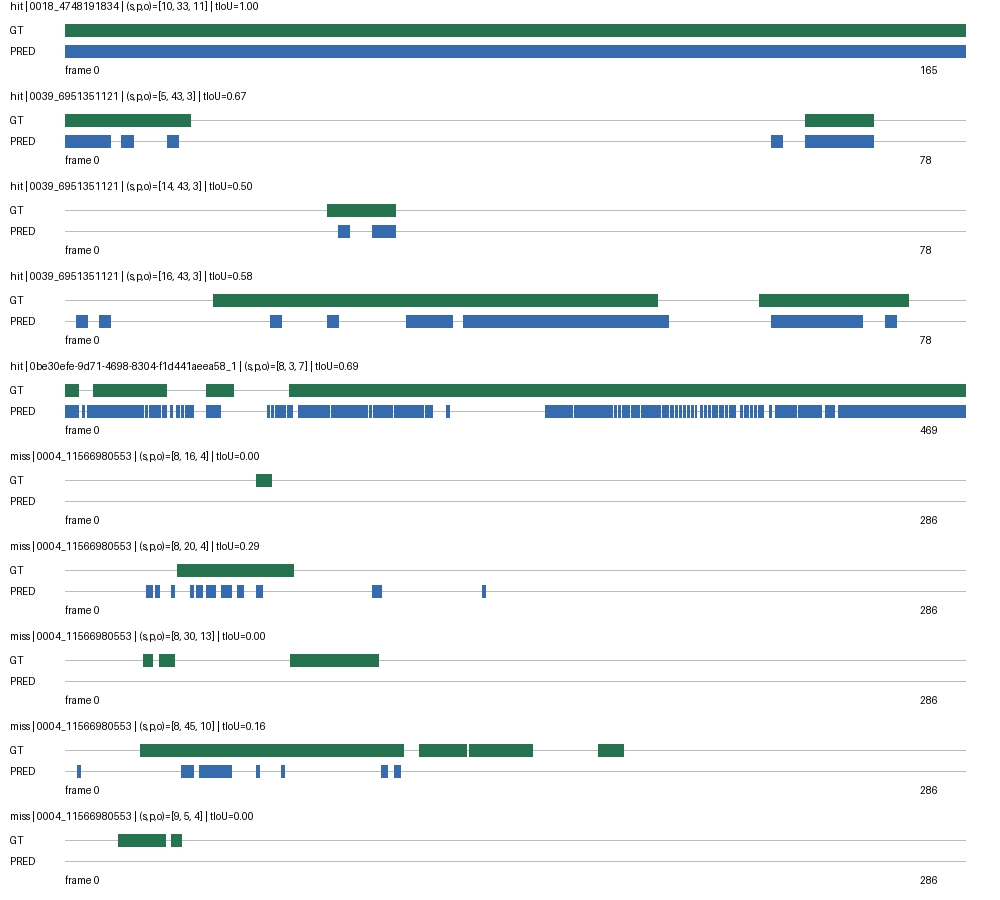
\includegraphics[width=.80\linewidth]{case_timelines.png}
\caption{Đoạn chuẩn (GT, xanh lá) và đoạn dự đoán (PRED, xanh dương) của Static GAT seed 17. Mười trường
hợp được lấy theo thứ tự video và bộ ba trong mỗi nhóm trúng hoặc bỏ sót.
Mỗi hàng có trục frame riêng.}\label{fig:timeline}
\end{figure}

\end{document}
